\documentclass[11pt,a4paper]{article}
\usepackage[T1]{fontenc}
\usepackage[utf8]{inputenc}
\usepackage{libertinus}
\usepackage[a4paper,margin=27mm,headheight=15pt]{geometry}
\usepackage{microtype}
\usepackage{amsmath,amssymb,amsthm,mathtools}
\usepackage{booktabs,array,longtable}
\usepackage{graphicx}
\usepackage{enumitem}
\usepackage{xurl}
\usepackage[hidelinks]{hyperref}
\usepackage[nameinlink,noabbrev]{cleveref}
\usepackage{fancyhdr}
\usepackage{listings}
\hypersetup{pdftitle={Entropic Edgeworth Expansions for Geometric Uniform Laws},pdfauthor={Research manuscript prepared with ChatGPT},pdfsubject={Proof of a ProveIt entropy conjecture, Renyi extensions, and finite-prefix asymptotics},pdfkeywords={Fabius function, Rvachev up-function, relative entropy, Renyi divergence, Edgeworth expansion, geometric uniforms}}
\pagestyle{fancy}
\fancyhf{}
\fancyhead[L]{\small Geometric uniform laws}
\fancyhead[R]{\small Entropic Edgeworth expansions}
\fancyfoot[C]{\thepage}
\setlength{\parindent}{1.2em}
\setlength{\parskip}{3pt}
\setlist[enumerate]{itemsep=4pt,topsep=5pt}
\numberwithin{equation}{section}
\newtheorem{theorem}{Theorem}[section]
\newtheorem{lemma}[theorem]{Lemma}
\newtheorem{proposition}[theorem]{Proposition}
\newtheorem{corollary}[theorem]{Corollary}
\theoremstyle{definition}
\newtheorem{definition}[theorem]{Definition}
\newtheorem{problem}[theorem]{Research question}
\theoremstyle{remark}
\newtheorem{remark}[theorem]{Remark}
\newcommand{\E}{\mathbb E}
\newcommand{\PP}{\mathbb P}
\newcommand{\R}{\mathbb R}
\newcommand{\N}{\mathbb N}
\newcommand{\eps}{\varepsilon}
\newcommand{\Var}{\operatorname{Var}}
\newcommand{\sinc}{\operatorname{sinc}}
\newcommand{\KL}{D}
\newcommand{\renyi}{D_{\alpha}}
\newcommand{\Normal}{\mathcal N}
\newcommand{\He}{H}
\newcommand{\dd}{\,dx}
\newcommand{\co}[2]{[#1^{#2}]}
\DeclareMathOperator{\supp}{supp}
\newcommand{\repo}{\texttt{ProveIt}}
\newcommand{\commit}{\nolinkurl{6c9175a54bcaad3bfc2d416257d2b7d3dff2c1e0}}
\lstset{basicstyle=\ttfamily\small,columns=fullflexible,breaklines=true,frame=single,showstringspaces=false}

\title{\bfseries Entropic Edgeworth Expansions\\for Geometric Uniform Laws\\[7pt]
\large A proof of a ProveIt conjecture, R\'enyi extensions,\\and uniform finite-prefix asymptotics}
\author{Research manuscript prepared with ChatGPT}
\date{28 September 2026}

\begin{document}
\maketitle
\begin{abstract}
Let $U_0,U_1,\ldots$ be independent uniforms on $[-1,1]$, and put
$X_q=(1-q)\sum_{j\ge0}q^jU_j$. At $q=1/2$ its density is the Rvachev
up-function. We prove the all-orders entropic Edgeworth conjecture stated in the
\repo\ manuscript \emph{Exact Information Geometry and New Frontiers for the
Fabius--Rvachev System}. With $Z_q=X_q/\sqrt{\Var(X_q)}$ and
$\eps=1-q$, the Gaussian entropy deficit satisfies
\[
 D(Z_q\|\Normal(0,1))
 =\frac3{100}\eps^2+\frac{33}{500}\eps^3
  +\frac{427297}{4410000}\eps^4+O(\eps^5),
\]
and has a rational-coefficient expansion to every order, with a genuine
$O_N(\eps^{N+1})$ remainder after degree $N$. The proof supplies the missing
uniform tail argument: subgaussianity and unimodality give a polynomial Gaussian
density-ratio envelope, while a block of comparable geometric scales gives
exponentially small high-frequency Fourier tails. These estimates turn arbitrary
absolute density expansions into nonlinear information expansions without
logarithmic losses. We also prove all-orders expansions for every fixed positive
R\'enyi order, uniformly on compact order intervals, and a two-parameter theorem
for finite prefixes with $q^{2m}$ bounded away from one. Exact coefficient code,
floating-point diagnostics, a proof-dependency audit, and further research
questions accompany the manuscript.
\end{abstract}

\noindent\textbf{Status.} The results below are conventional mathematical proofs,
not Lean-checked results. The main claim is a resolution of the explicitly
identified repository conjecture at the inspected commit. No claim of priority
for the general theory of entropic Edgeworth expansions, or of independent
peer review, is made.

\newpage
\tableofcontents
\newpage

\section{The repository question and the scope of the result}
\label{sec:scope}

\subsection{A precise question rather than an unspecified breakthrough}

The Fabius-function part of \repo\ contains both formal mathematics and research
manuscripts. The relevant source for this article is the manuscript with the
repository-relative path
\begin{quote}\small\ttfamily\raggedright
Analysis/FabiusFunction/docs/\allowbreak
semi-formalized-research-frontiers/\allowbreak
drafts/inverse-and-sampling/\allowbreak
fabius\_information\_frontier/\allowbreak
fabius\_information\_frontier.tex.
\end{quote}
At commit \commit, its conjecture with label
\texttt{conj:entropic-edgeworth} asks whether the formal expansion
\begin{equation}
 \Delta(q)=\frac3{100}(1-q)^2+\frac{33}{500}(1-q)^3+O((1-q)^4)
 \label{eq:original}
\end{equation}
is a genuine asymptotic expansion, and whether it extends to all orders with
explicit rational coefficients. The accompanying explanation identifies the
remaining problem as uniform moderate- and far-tail control, not formal
coefficient algebra \cite{repo}.

We prove that assertion, including its all-orders remainder. The R\'enyi and
finite-prefix results below are extensions of the same argument. The result is
substantive within the repository's information-theoretic research program:
it upgrades the stated conjecture to a proof and makes the higher coefficients
usable with a justified asymptotic error order. It should not be confused with a
claim to have originated entropic Edgeworth theory itself.

\subsection{Relation to established literature}

Arias de Reyna's work provides a primary reference for the Fabius function and
its arithmetic conventions \cite{arias}. For the information-theoretic
background, Bobkov, Chistyakov, and G\"otze established entropic Edgeworth
expansions for normalized sums of independent identically distributed random
variables under moment hypotheses \cite{bcg2013}. Their work on R\'enyi
divergence treats stronger normal-approximation distances and exact convergence
rates \cite{bcg2016}; their later account discusses the role of strict
subgaussianity, including infinite-order divergence \cite{bcg2025}.

These are close antecedents, not results being rediscovered without attribution.
Here the summands have a geometric triangular-array structure and there are
infinitely many of them. In the finite-prefix extension, the number of summands
and the geometric ratio vary simultaneously. Rather than silently applying an
iid theorem, we prove the Fourier and tail estimates needed for this family.
All analytic steps specific to the present result are supplied below.

\subsection{What is, and is not, asserted}

The manuscript proves a repository-specific conjecture and records extensions
whose exact formulation was not found in the targeted source inspection.
That inspection was not an exhaustive review of every repository file or of all
published literature. General transform methods, cumulant expansions, Hermite
orthogonality, and entropy renormalization are established techniques.

The proofs do not use unverified mathematical claims from other parts of the
repository. In particular, they require no large-cardinal, computability,
polynomial-solvability, or surreal-number result. The exact cumulant identity is
rederived. The symbolic program checks finite coefficient identities; it does
not certify the analytic remainder theorem. No repository file was modified,
and no Lean build was performed for this article.

\section{Laws, normalization, and the main theorem}
\label{sec:main}

Let $U_j$ be independent and uniformly distributed on $[-1,1]$. For $0<q<1$,
set
\begin{equation}
 X_q=(1-q)\sum_{j=0}^{\infty}q^jU_j,
 \qquad
 \sigma_q^2=\Var(X_q)=\frac{1-q}{3(1+q)}.
 \label{eq:law}
\end{equation}
The series converges absolutely for every realization. The standardized law is
\begin{equation}
 Z_q=\frac{X_q}{\sigma_q}
 =\sqrt{3(1-q^2)}\sum_{j=0}^{\infty}q^jU_j.
 \label{eq:standardized}
\end{equation}
At $q=1/2$, $X_q$ has the centered Rvachev density, so this family contains the
classical Fabius--Rvachev system while allowing a near-Gaussian regime.

Write
\begin{equation}
 \phi(x)=\frac{e^{-x^2/2}}{\sqrt{2\pi}},
 \qquad
 h(p)=-\int_{\R}p(x)\log p(x)\dd.
\end{equation}
All logarithms are natural and all information quantities are in nats. For a
variance-one, mean-zero density $p$,
\begin{equation}
 D(p\|\phi)=\int p\log\frac p\phi
 =\frac12\log(2\pi e)-h(p).
 \label{eq:entropy-deficit}
\end{equation}
We use $0\log0=0$ throughout.

\begin{theorem}[All-orders resolution of the repository conjecture]
\label{thm:main}
There is a uniquely determined sequence of rational numbers $(d_n)_{n\ge2}$
such that, for every integer $N\ge2$, there are constants $C_N<\infty$ and
$\eps_N>0$ for which
\begin{equation}
 \left|D(Z_{1-\eps}\|\phi)-\sum_{n=2}^{N}d_n\eps^n\right|
 \le C_N\eps^{N+1}
 \qquad(0<\eps<\eps_N).
 \label{eq:main-estimate}
\end{equation}
Every coefficient is obtained by finite rational operations on Bernoulli
numbers and Gaussian polynomial moments. The first seven are
\begin{align}
 d_2&=\frac3{100},&
 d_3&=\frac{33}{500},&
 d_4&=\frac{427297}{4410000},\notag\\
 d_5&=\frac{2612237}{27562500},&
 d_6&=-\frac{257501}{55566000},&
 d_7&=-\frac{462000293}{1653750000},\notag\\
 d_8&=-\frac{216929586074851}{392203350000000}.
 \label{eq:coefficients}
\end{align}
\end{theorem}

The sign changes in \eqref{eq:coefficients} are not a contradiction: the positive
quadratic term controls the deficit near $q=1$. The theorem is an asymptotic
statement, not a claim that the resulting infinite series converges.

To prove the theorem efficiently, we include finite prefixes from the outset.
For $m\in\{1,2,\ldots\}\cup\{\infty\}$, let
\begin{equation}
 \rho=q^{2m},\qquad
 \beta=\sqrt{\frac{3(1-q^2)}{1-\rho}},\qquad
 Z_{q,m}=\beta\sum_{j=0}^{m-1}q^jU_j,
 \label{eq:finite-law}
\end{equation}
where $q^{2\infty}=0$ and an upper limit $\infty-1$ means an infinite sum.
Then $Z_{q,\infty}=Z_q$ and $\Var(Z_{q,m})=1$.

\begin{definition}[Admissible uniform regime]
Fix $\rho_0\in(0,1)$. An admissible pair $(q,m)$ satisfies
$q\uparrow1$ and $0\le\rho=q^{2m}\le\rho_0$.
Unless stated otherwise, uniform estimates below are over all such pairs.
\end{definition}

For a finite prefix, $\rho$ is not an independent continuous parameter of the
probability law. In coefficient extraction it is held fixed as an auxiliary
algebraic parameter; the resulting formulas are evaluated only at admissible
pairs. No differentiation of $m$ is involved.

\section{Cumulants and polynomial coefficients}
\label{sec:coeff-setup}

The characteristic function of $Z_{q,m}$ is
\begin{equation}
 \chi_{q,m}(t)=\prod_{j=0}^{m-1}\sinc(\beta q^jt),
 \qquad \sinc v=\begin{cases}\sin(v)/v,&v\ne0,\\1,&v=0.\end{cases}
 \label{eq:characteristic}
\end{equation}
The moment generating function of $U_j$ is $\sinh z/z$. Its logarithm has the
convergent local expansion
\begin{equation}
 \log\frac{\sinh z}{z}
 =\sum_{r\ge1}\frac{2^{2r}B_{2r}}{2r}\frac{z^{2r}}{(2r)!},
 \qquad |z|<\pi,
 \label{eq:uniform-logmgf}
\end{equation}
where $B_2=1/6$, $B_4=-1/30$, and $B_6=1/42$. One way to obtain this
identity is to integrate the Bernoulli expansion of
$\coth z-1/z$. Odd cumulants vanish by symmetry.

\begin{proposition}[Exact finite- and infinite-prefix cumulants]
\label{prop:cumulants}
For $r\ge2$, the standardized cumulant of order $2r$ is
\begin{equation}
 \lambda_{2r}(q,\rho)
 =\frac{3^r2^{2r}B_{2r}}{2r}
 \frac{(1-q^2)^{r-1}}{1+q^2+\cdots+q^{2r-2}}
 \frac{1-\rho^r}{(1-\rho)^r}.
 \label{eq:cumulants}
\end{equation}
It is analytic in $\eps=1-q$ near zero, uniformly for
$\rho\in[0,\rho_0]$, and is $O_r(\eps^{r-1})$ there.
\end{proposition}
\begin{proof}
Cumulants add under independence and scale homogeneously. Thus the cumulant is
\[
 \frac{2^{2r}B_{2r}}{2r}\,
 \beta^{2r}\sum_{j=0}^{m-1}q^{2rj}
 =\frac{2^{2r}B_{2r}}{2r}\,
 \beta^{2r}\frac{1-\rho^r}{1-q^{2r}}.
\]
Insert \eqref{eq:finite-law} and factor $1-q^{2r}$.
The denominator $1+q^2+\cdots+q^{2r-2}$ equals $r$ at $q=1$, and
$1-\rho$ stays bounded away from zero. These observations prove the analytic
and uniform-order assertions. The calculation for $r=1$ gives variance one.
\end{proof}

Let the probabilists' Hermite polynomials be defined by
\begin{equation}
 e^{tx-t^2/2}=\sum_{k\ge0}H_k(x)\frac{t^k}{k!}.
 \label{eq:hermite}
\end{equation}
For a polynomial in a formal variable $z$, define the linear map
\begin{equation}
 \mathcal H(z^k)=H_k(x).
 \label{eq:hermite-map}
\end{equation}
It is important that $\mathcal H$ is linear, not multiplicative.

Define finite polynomials
\begin{align}
 A_j(z;\rho)
 &=\co{\eps}{j}\sum_{r=2}^{j+1}
   \lambda_{2r}(1-\eps,\rho)\frac{z^{2r}}{(2r)!},
 \label{eq:Aj}\\
 E_n(z;\rho)
 &=\co{\eps}{n}\exp\left(\sum_{j\ge1}\eps^jA_j(z;\rho)\right),
 \qquad E_0=1,\label{eq:En}\\
 P_n(x;\rho)&=\mathcal H E_n(z;\rho).
 \label{eq:Pn}
\end{align}
The recurrence
\begin{equation}
 nE_n=\sum_{j=1}^{n}jA_jE_{n-j}
 \label{eq:recurrence}
\end{equation}
is a convenient exact algorithm. We have $\deg E_n\le4n$; every nonzero
monomial in $E_n$, $n\ge1$, has even degree at least four. Consequently,
\begin{equation}
 \E P_n(G;\rho)=0,
 \qquad \E\bigl[G^2P_n(G;\rho)\bigr]=0,
 \qquad G\sim\Normal(0,1).
 \label{eq:normalizations}
\end{equation}
These identities encode normalization and the unchanged variance.

For later use put
\begin{equation}
 A=\frac{1+\rho}{1-\rho},\qquad
 B=\frac{1+\rho+\rho^2}{(1-\rho)^2}.
 \label{eq:AB}
\end{equation}
Direct expansion of \eqref{eq:cumulants} gives
\begin{align}
 P_1&=-\frac A{20}H_4,\label{eq:P1}\\
 P_2&=-\frac A{40}H_4+\frac{4B}{315}H_6
       +\frac{A^2}{800}H_8.
 \label{eq:P2}
\end{align}
The original infinite law corresponds to $A=B=1$.

\section{Uniform Fourier smoothing}
\label{sec:fourier}

The main obstacle to using the preceding algebra is not the coefficients. It is
justifying Fourier inversion and its remainder uniformly as $q$ approaches one.
The following estimates handle both finite and infinite prefixes.

\begin{lemma}[A low-frequency sinc bound]
\label{lem:sinc}
For $|v|\le1$,
\begin{equation}
 0<\sinc v\le e^{-v^2/6}.
 \label{eq:sinc-bound}
\end{equation}
Consequently, for $|t|\le\beta^{-1}$,
\begin{equation}
 |\chi_{q,m}(t)|\le e^{-t^2/2}.
 \label{eq:low-frequency}
\end{equation}
\end{lemma}
\begin{proof}
For $0<v\le1$ let
$F(v)=(3-v^2)\sin v-3v\cos v$. Then
$F'(v)=v(\sin v-v\cos v)$, and the derivative of
$\sin v-v\cos v$ is $v\sin v\ge0$. Therefore $F(v)\ge0$, which is
$1/v-\cot v\ge v/3$. Integrating yields
$\log(\sin v/v)\le-v^2/6$. Evenness treats negative $v$.
Finally, $\sum_{j<m}\beta^2q^{2j}=3$, so multiplication of the individual
bounds gives \eqref{eq:low-frequency}.
\end{proof}

\begin{lemma}[Comparable-scale block]
\label{lem:block}
For every fixed $\rho_0<1$ there are constants $c,d>0$ such that, for all
sufficiently small admissible $\eps$, the sum in \eqref{eq:finite-law} has at
least $K=\lfloor c/\eps\rfloor$ terms, and
\begin{equation}
 q^j\ge d\qquad(0\le j<K).
 \label{eq:block}
\end{equation}
Also $\beta\asymp\sqrt\eps$, with constants depending only on $\rho_0$.
\end{lemma}
\begin{proof}
For $q\ge1/2$ we have $\eps\le-\log q\le2\eps$. If $m<\infty$,
\[
 m=\frac{-\log\rho}{2(-\log q)}
 \ge\frac{-\log\rho_0}{4\eps}.
\]
Choose $c>0$ smaller than $-\log\rho_0/8$. For $j<K$,
$q^j\ge e^{-2\eps K}\ge e^{-2c}$, so $d=e^{-2c}$ works.
The infinite case needs no bound on $m$. The comparison for $\beta$ follows
from $\eps\le1-q^2\le2\eps$ and $1-\rho\in[1-\rho_0,1]$.
\end{proof}

\begin{lemma}[Exponentially small high-frequency integral]
\label{lem:high}
For each fixed nonnegative integer $k$, there are positive constants $C,c$
such that
\begin{equation}
 \int_{|t|>\beta^{-1}}|t|^k|\chi_{q,m}(t)|\,dt
 \le C\eps^{-(k+1)/2}e^{-c/\eps}.
 \label{eq:high-frequency}
\end{equation}
In particular, all fixed polynomially weighted Fourier $L^1$ norms are
uniformly bounded for sufficiently small $\eps$.
\end{lemma}
\begin{proof}
For the $d$ in \cref{lem:block},
\[
 \eta:=\sup_{|v|\ge d}|\sinc v|<1.
\]
Indeed, $|\sin v|<|v|$ for $v\ne0$, continuity controls a compact annulus,
and $|\sinc v|\le1/|v|$ controls infinity.
Fix an integer $L>k+1$ and take $\eps$ small enough that $K>2L$.
For $|t|>\beta^{-1}$, the arguments of the first $K$ factors have absolute
value at least $d$. Use $|\sinc v|\le1/|v|$ on the first $L$ factors,
$|\sinc v|\le\eta$ on the next $K-L$, and $|\sinc v|\le1$ on the
remaining factors. This gives
\begin{equation}
 |\chi_{q,m}(t)|
 \le(\beta|t|)^{-L}q^{-L(L-1)/2}\eta^{K-L}.
 \label{eq:pointwise-high}
\end{equation}
The fixed power of $q^{-1}$ is bounded, and
$\eta^{K-L}\le C e^{-c/\eps}$. Integration of $t^{k-L}$ from
$\beta^{-1}$ to infinity gives $C\beta^{-k-1}e^{-c/\eps}$, proving
\eqref{eq:high-frequency}. The remaining Fourier interval is bounded by
\cref{lem:sinc}.
\end{proof}

\begin{corollary}[Uniformly bounded densities]
\label{cor:density-exists}
The admissible laws have continuous densities $p_{q,m}$ for sufficiently small
$\eps$, and $\sup_{q,m}\|p_{q,m}\|_\infty<\infty$.
For each fixed derivative order, the corresponding derivatives exist and are
uniformly bounded after reducing the admissible upper bound on $\eps$.
\end{corollary}
\begin{proof}
Apply Fourier inversion and differentiation under its absolutely convergent
integral, using \cref{lem:high}. For a finite prefix the required number of
convolutions is available because $m\to\infty$ in the admissible regime.
\end{proof}

\section{A Gaussian envelope that survives the endpoints}
\label{sec:envelope}

A uniform density expansion in absolute error alone is not the needed entropy
estimate: division by $\phi$ amplifies that error in the tails. The following
elementary argument provides the missing nonlinear control.

\begin{lemma}[Exact-variance subgaussianity]
\label{lem:subgaussian}
For every finite or infinite law in \eqref{eq:finite-law} and every real $t$,
\begin{equation}
 \E e^{tZ_{q,m}}\le e^{t^2/2}.
 \label{eq:subgaussian}
\end{equation}
Hence $\PP(Z_{q,m}\ge x)\le e^{-x^2/2}$ for $x\ge0$.
\end{lemma}
\begin{proof}
The coefficient inequality $(2j+1)!\ge6^j j!$ gives, for real $v$,
\[
 \frac{\sinh v}{v}
 =\sum_{j\ge0}\frac{v^{2j}}{(2j+1)!}
 \le\sum_{j\ge0}\frac{v^{2j}}{6^j j!}=e^{v^2/6}.
\]
The factorial inequality follows by induction: its successive ratio is
$(2j+3)(2j+2)/(6(j+1))=(2j+3)/3\ge1$.
Multiplication of these moment-generating-function bounds yields
\eqref{eq:subgaussian}, since the sum of squared interval half-widths is three.
For the infinite sum, bounded convergence applies to the exponential of the
absolutely convergent series at fixed $q$. Chernoff's bound with $t=x$ gives
the stated tail estimate.
\end{proof}

\begin{lemma}[Unimodality]
\label{lem:unimodal}
The density $p_{q,m}$ is even and nonincreasing on $[0,\infty)$.
\end{lemma}
\begin{proof}
Convolution of an even, nonincreasing-on-the-positive-axis function $f$ with
a uniform density on $[-a,a]$ is
$g(x)=(2a)^{-1}\int_{x-a}^{x+a}f(u)\,du$. Wherever its derivative is
represented by endpoint values,
\[
 g'(x)=\frac{f(x+a)-f(x-a)}{2a}\le0\qquad(x\ge0),
\]
because $|x+a|\ge|x-a|$ and $f$ is even. The same conclusion follows by
integration when $f$ has jumps. Induction proves the finite-convolution
assertion. For the infinite sum, finite-prefix densities converge uniformly
once two fixed initial factors give an integrable Fourier majorant. Their
limit is the density of the infinite sum and preserves evenness and
monotonicity.
\end{proof}

\begin{theorem}[Polynomial Gaussian density-ratio envelope]
\label{thm:envelope}
For fixed $\rho_0<1$ there is $C<\infty$ such that all sufficiently small
admissible $\eps$ satisfy
\begin{equation}
 0\le\frac{p_{q,m}(x)}{\phi(x)}\le C(1+|x|)
 \qquad(x\in\R).
 \label{eq:envelope}
\end{equation}
\end{theorem}
\begin{proof}
If $x\ge1$, unimodality and \cref{lem:subgaussian} give
\[
 \frac1x p_{q,m}(x)
 \le\int_{x-1/x}^{x}p_{q,m}(u)\,du
 \le\PP(Z_{q,m}\ge x-1/x)
 \le e^{-(x-1/x)^2/2}.
\]
Therefore
\[
 p_{q,m}(x)\le ex e^{-x^2/2},
 \qquad
 \frac{p_{q,m}(x)}{\phi(x)}\le e\sqrt{2\pi}\,x.
\]
Use evenness on the negative axis. On $[-1,1]$, use the uniform density
bound in \cref{cor:density-exists} and the positive minimum of $\phi$ there.
\end{proof}

This bound is valid where the density is extremely small and where it is
exactly zero outside its support. It is stronger for the present purpose than
an estimate confined to a fixed compact interval. No endpoint asymptotic for
the Fabius function, and no lower bound on $p_{q,m}$ in the far tails, is needed.

\section{All-orders density expansions}
\label{sec:density-expansion}

\begin{theorem}[Uniform absolute Edgeworth expansion]
\label{thm:density-expansion}
For every integer $M\ge0$, uniformly over admissible pairs,
\begin{equation}
 \sup_{x\in\R}\left|
 p_{q,m}(x)-\phi(x)\left(1+\sum_{n=1}^{M}\eps^nP_n(x;\rho)\right)
 \right|\le C_{M,\rho_0}\eps^{M+1}.
 \label{eq:density-expansion}
\end{equation}
The same assertion holds after any fixed number of derivatives in $x$, with
the corresponding derivative of the displayed approximating density.
\end{theorem}
\begin{proof}
The case $M=0$ is included in the following proof. On a neighborhood of the
origin, the logarithm of \eqref{eq:characteristic} is
\[
 \log\chi_{q,m}(t)
 =-\frac{t^2}{2}+\sum_{r\ge2}
  \lambda_{2r}(q,\rho)\frac{(it)^{2r}}{(2r)!}.
\]
Truncate the logarithm of each sinc factor after degree $2M+2$.
For arguments bounded by, say, $1/2$, its remainder is bounded by a constant
times the $(2M+4)$th power of the argument. Summing over the factors is
legitimate, including in the infinite case, because
\begin{equation}
 \sum_{j<m}(\beta q^j)^{2M+4}
 \le\beta^{2M+2}\sum_{j<m}(\beta q^j)^2
 =3\beta^{2M+2}=O(\eps^{M+1}).
 \label{eq:log-remainder}
\end{equation}
Taylor-expand the finitely many rational cumulants in $\eps$ through degree
$M$, holding $\rho$ fixed. Their remainders are uniform on
$[0,\rho_0]$ by \cref{prop:cumulants}. Thus
\begin{equation}
 \log\chi_{q,m}(t)
 =-\frac{t^2}{2}+\sum_{j=1}^{M}\eps^jA_j(it;\rho)
 +O_M\!\left(\eps^{M+1}(1+|t|^{2M+4})\right)
 \label{eq:log-local}
\end{equation}
whenever $\beta|t|$ is sufficiently small.

Choose $\delta=1/(8(M+2))$ and first restrict to
$|t|\le\eps^{-\delta}$. In this region
$\eps(1+|t|^4)\to0$. Since $\deg A_j\le2j+2\le4j$, expanding the
exponential in \eqref{eq:log-local} and using \eqref{eq:En} yields
\begin{align}
 \Bigl|\chi_{q,m}(t)
 -e^{-t^2/2}\sum_{n=0}^{M}\eps^nE_n(it;\rho)\Bigr|
 &\le C_M\eps^{M+1}(1+|t|^4)^{M+1}e^{-t^2/2}.
 \label{eq:local-fourier-error}
\end{align}
For clarity, this is an ordinary finite Taylor estimate, not a formal equality:
the correction in the exponent is uniformly small on this region, its
exponential has a bounded Taylor remainder, and every omitted monomial has
$\eps$-weight at least $M+1$. The logarithmic remainder in
\eqref{eq:log-local} fits the same polynomial bound.

On $\eps^{-\delta}<|t|\le\beta^{-1}$, use
\eqref{eq:low-frequency} for the actual characteristic function and a
Gaussian times a fixed polynomial for its approximation. Their integrals,
with any fixed additional factor $|t|^k$, are smaller than every power of
$\eps$. On $|t|>\beta^{-1}$, use \cref{lem:high} and again the Gaussian
bound for the approximating polynomial. It follows that
\begin{equation}
 \int_{\R}|t|^k\left|
 \chi_{q,m}(t)-e^{-t^2/2}\sum_{n=0}^{M}\eps^nE_n(it;\rho)
 \right|dt\le C_{M,k}\eps^{M+1}.
 \label{eq:fourier-L1-error}
\end{equation}

Finally,
\[
 \int_{\R}e^{itx}\phi(x)H_j(x)\dd=(it)^je^{-t^2/2},
\]
as follows directly from \eqref{eq:hermite}. Fourier inversion transforms
\eqref{eq:fourier-L1-error} with $k=0$ into
\eqref{eq:density-expansion}; the other $k$ give the derivative version.
\end{proof}

\begin{remark}[The approximation is not a density everywhere]
An Edgeworth polynomial times $\phi$ can be negative in a remote region. No
step above asserts otherwise. In the nonlinear argument below it is used as
a density ratio only on an expanding central interval where it is close to
one; in the tails only the true density and the envelope are used.
\end{remark}

\section{From local expansions to nonlinear information}
\label{sec:transfer}

The loss of powers of $\log(1/\eps)$ is a common pitfall in an informal
entropy calculation. We avoid it by proving a deeper density expansion than
the final information order requires, and by integrating polynomial errors
against the Gaussian rather than bounding them by their central-interval
suprema.

\begin{lemma}[Nonlinear transfer with an exact power remainder]
\label{lem:transfer}
Suppose a family of densities $p_\eps$ has the uniform expansions
\eqref{eq:density-expansion} to every order, with polynomial coefficients
$P_n$, and the envelope \eqref{eq:envelope}. Let $\Psi:[0,\infty)\to\R$
be continuous, analytic near one, and satisfy
\begin{equation}
 \Psi(1)=\Psi'(1)=0,
 \qquad |\Psi(r)|\le C(1+r^b)
 \quad(r\ge0)
 \label{eq:psi-assumptions}
\end{equation}
for some fixed $b$. Then, for every $N\ge2$,
\begin{equation}
 \int_{\R}\phi(x)\Psi\!\left(\frac{p_\eps(x)}{\phi(x)}\right)\dd
 =\sum_{n=2}^{N}c_n\eps^n+O_N(\eps^{N+1}),
 \label{eq:transfer}
\end{equation}
where $c_n$ is obtained by substituting
$1+\sum_{j\ge1}\eps^jP_j$ into the Taylor series of $\Psi$ and integrating
coefficientwise against $\phi$. The estimate is uniform over auxiliary compact
parameter sets whenever all the hypotheses and local Taylor bounds are uniform.
\end{lemma}
\begin{proof}
Fix $N$. Let
\begin{equation}
 T=\sqrt{B\log(1/\eps)},\qquad B=4(N+2),\qquad M=3N+6.
 \label{eq:cutoffs}
\end{equation}
By the envelope and polynomial growth of $\Psi$, the part of the integral
with $|x|>T$ is bounded by a fixed Gaussian polynomial tail. Hence it is
$O(\eps^{N+2})$. The same is true for the tails of all finitely many
polynomial coefficients needed below. Indeed, a fixed power of $T$ times
$e^{-T^2/2}=\eps^{2N+4}$ is $O(\eps^{N+2})$.

On $|x|\le T$, $\phi(x)\ge(2\pi)^{-1/2}\eps^{B/2}$.
Use the density expansion at order $M$, not merely at order $N$. Division by
$\phi$ gives
\begin{equation}
 \frac{p_\eps(x)}{\phi(x)}
 =1+\sum_{j=1}^{M}\eps^jP_j(x)+O(\eps^{M+1-B/2})
 =1+\sum_{j=1}^{M}\eps^jP_j(x)+O(\eps^{N+3}).
 \label{eq:central-ratio}
\end{equation}
All terms on the right after one tend uniformly to zero on this interval.
Put $u_N(x)=\sum_{j=1}^{N}\eps^jP_j(x)$. The difference between the
ratio in \eqref{eq:central-ratio} and $1+u_N$ is bounded by
\begin{equation}
 C\eps^{N+1}Q(x)+C\eps^{N+3}
 \label{eq:replace-error}
\end{equation}
for a fixed polynomial bound $Q\ge0$. Since $\Psi'$ is bounded in a fixed
neighborhood of one, replacing the true ratio by $1+u_N$ changes the central
integral by $O(\eps^{N+1})$: integrate $Q$ against $\phi$ instead of taking
its supremum on $[-T,T]$.

Taylor-expand $\Psi(1+u_N)$ through degree $N$ in $u_N$. Its remainder is
bounded by $C|u_N|^{N+1}$. There is a fixed polynomial bound $Q_N$ with
$|u_N|\le\eps Q_N$, so the integrated remainder is
$O(\eps^{N+1})$. In the remaining finite polynomial, every monomial of
$\eps$-weight greater than $N$ likewise contributes $O(\eps^{N+1})$.
Restoring the coefficient integrals from $[-T,T]$ to $\R$ costs only the
already bounded Gaussian tails. This proves \eqref{eq:transfer}.
\end{proof}

For relative entropy, the correct affine-renormalized integrand is
\begin{equation}
 \Psi_1(r)=r\log r-r+1,
 \qquad
 D(p\|\phi)=\int\phi\,\Psi_1(p/\phi).
 \label{eq:KL-psi}
\end{equation}
The equality uses $\int(p-\phi)=0$. The function is continuous at zero,
with $\Psi_1(0)=1$, and has polynomial growth. Around one,
\begin{equation}
 \Psi_1(1+u)=\sum_{k\ge2}\frac{(-1)^k}{k(k-1)}u^k.
 \label{eq:KL-series}
\end{equation}

\begin{proof}[Proof of \cref{thm:main}]
Apply \cref{lem:transfer} with $\rho=0$ and $\Psi=\Psi_1$, using
\cref{thm:density-expansion,thm:envelope}. The coefficient algorithm is
\eqref{eq:Aj}--\eqref{eq:recurrence} followed by \eqref{eq:KL-series}.
All Gaussian moments of polynomials with rational coefficients are rational.
The Bernoulli dependence comes from \eqref{eq:cumulants}. The values in
\eqref{eq:coefficients} are calculated below and in the accompanying exact
program. Uniqueness of asymptotic coefficients follows successively by dividing
the difference of two expansions by the first possibly nonzero power of
$\eps$ and taking $\eps\downarrow0$.
\end{proof}

\section{Explicit coefficients and exact arithmetic}
\label{sec:explicit}

Let
\begin{equation}
 U(\eps,x;\rho)=\sum_{j\ge1}\eps^jP_j(x;\rho)
 \label{eq:formal-U}
\end{equation}
be a formal series. The Shannon coefficients are
\begin{equation}
 d_n(\rho)=\sum_{k=2}^{n}\frac{(-1)^k}{k(k-1)}
 \sum_{\substack{j_1+\cdots+j_k=n\\j_i\ge1}}
 \E\!\left[\prod_{i=1}^{k}P_{j_i}(G;\rho)\right].
 \label{eq:coefficient-formula}
\end{equation}
Only $P_1,\ldots,P_{n-1}$ are needed. In particular, the linear error in the
density expansion does not contribute directly to the information coefficient.

\subsection{The first two nonzero terms}

Using \eqref{eq:P1}--\eqref{eq:P2} and Hermite orthogonality,
\begin{align}
 \E P_1^2&=\frac{3A^2}{50},&
 \E(P_1P_2)&=\frac{3A^2}{100},&
 \E P_1^3&=-\frac{27A^3}{125}.
 \label{eq:low-moments}
\end{align}
Therefore
\begin{equation}
 d_2(\rho)=\frac{3A^2}{100},\qquad
 d_3(\rho)=\frac{3A^2}{100}+\frac{9A^3}{250}.
 \label{eq:prefix-low}
\end{equation}
At $\rho=0$, these are exactly the two coefficients conjectured in
\eqref{eq:original}.

\subsection{A useful invariant fourth-order formula}

Suppress the parameters in the cumulants and assign asymptotic weight $r-1$
to $\lambda_{2r}$. Through weight four, the entropy is
\begin{align}
 D(p_{q,m}\|\phi)
 ={}&\frac{\lambda_4^2}{48}-\frac{\lambda_4^3}{48}
   +\frac{\lambda_6^2}{1440}
   -\frac{\lambda_4^2\lambda_6}{72}
   +\frac{89\lambda_4^4}{1152}
   +O(\eps^5).
 \label{eq:invariant-fourth}
\end{align}
This expression uses the exact cumulants at the actual parameters, not their
leading terms. For example, it automatically includes the higher powers of
$\eps$ hidden in $\lambda_4^2$.

Here is a direct check of the less immediate constants. The required Gaussian
Hermite moments are
\begin{equation}
 \E H_4^3=1728,\quad
 \E(H_4^2H_6)=11520,\quad
 \E(H_4^2H_8)=40320,\quad
 \E H_4^4=368064.
 \label{eq:hermite-values}
\end{equation}
Write the first two cumulant-weight parts of the density ratio as
\[
 u_1=aH_4,\qquad u_2=bH_6+\tfrac12a^2H_8,
 \quad a=\lambda_4/24,\quad b=\lambda_6/720.
\]
All weight-three terms in the ratio are orthogonal to $H_4$. Hence the
weight-four entropy contribution is
$\frac12\E u_2^2-\frac12\E(u_1^2u_2)+\frac1{12}\E u_1^4$.
Substitution of \eqref{eq:hermite-values} gives the last three terms of
\eqref{eq:invariant-fourth}.

It follows that the finite-prefix quartic coefficient is
\begin{equation}
 \boxed{\displaystyle
 d_4(\rho)=\frac{3A^2}{400}+\frac{27A^3}{500}
  +\frac{128B^2}{2205}-\frac{32A^2B}{175}
  +\frac{801A^4}{5000}.}
 \label{eq:prefix-fourth}
\end{equation}
Setting $A=B=1$ yields $427297/4410000$.

\subsection{Reproducible higher coefficients}

The supplied program \path{code/coefficients.py} uses only exact SymPy rational
arithmetic. It first expands the rational cumulants, constructs the $E_n$ by
\eqref{eq:recurrence}, applies the linear Hermite map, and evaluates the
Gaussian moments in \eqref{eq:coefficient-formula}. Gaussian integration is
implemented by
\begin{equation}
 \E G^{2j}=\frac{(2j)!}{2^j j!},\qquad \E G^{2j+1}=0.
 \label{eq:normal-moments}
\end{equation}
The output through degree eight is stored in
\path{data/exact_coefficients.json}. It also contains the intermediate Hermite
symbol polynomials and Gaussian product moments, allowing the calculation to be
inspected rather than merely trusted as a decimal fit.

The program separately constructs the R\'enyi coefficient polynomials and
checks their value at $\alpha=1$ against the Shannon calculation. It checks
normalization and variance identities for every constructed $P_n$. These
checks support the finite algebra in \eqref{eq:coefficients}; the analytic
proof remains \cref{sec:fourier,sec:envelope,sec:density-expansion,sec:transfer}.

\section{R\'enyi expansions at every fixed positive order}
\label{sec:renyi}

For $\alpha>0$, $\alpha\ne1$, define
\begin{equation}
 D_\alpha(p\|\phi)=\frac1{\alpha-1}
  \log\int_{\R}p(x)^\alpha\phi(x)^{1-\alpha}\dd,
 \label{eq:renyi}
\end{equation}
and put $D_1=D$. All these quantities are finite for the admissible laws:
\eqref{eq:envelope} bounds the integrand by a Gaussian times a polynomial.
This observation holds for $\alpha>1$ as well as for $0<\alpha<1$.

\begin{theorem}[All-orders positive-order R\'enyi expansion]
\label{thm:renyi}
For each $N\ge2$ and every compact interval
$K\subset(0,\infty)$,
\begin{equation}
 D_\alpha(p_{q,m}\|\phi)
 =\sum_{n=2}^{N}d_n(\alpha,\rho)\eps^n
  +O_{N,K,\rho_0}(\eps^{N+1}),
 \label{eq:renyi-expansion}
\end{equation}
uniformly for $\alpha\in K$ and admissible $(q,m)$. Each
$d_n(\alpha,\rho)$ is a polynomial in $\alpha$ of degree at most $n-1$,
with coefficients rational in $\rho$ and in the Bernoulli numbers.
At $\alpha=1$ it equals $d_n(\rho)$.
\end{theorem}
\begin{proof}
Use the affine-renormalized family
\begin{equation}
 \Psi_\alpha(r)=
 \frac{r^\alpha-1-\alpha(r-1)}{\alpha-1}
 \quad(\alpha\ne1),\qquad
 \Psi_1(r)=r\log r-r+1.
 \label{eq:tsallis-psi}
\end{equation}
It is continuous on $[0,\infty)$, with the continuous parameter extension at
$\alpha=1$. On a fixed neighborhood of $r=1$ all required Taylor bounds
are uniform for $\alpha\in K$. Polynomial growth is also uniform: near
$r=0$, factors of the form $r^a|\log r|$ are bounded when $a>0$, and for
large $r$ one can use a power greater than $\max K$.

By \cref{lem:transfer},
\[
 T_\alpha:=\int\phi\,\Psi_\alpha(p_{q,m}/\phi)
\]
has an all-orders expansion and is $O(\eps^2)$ uniformly. Since
$\int(p_{q,m}-\phi)=0$,
\begin{equation}
 D_\alpha(p_{q,m}\|\phi)
 =\frac{\log(1+(\alpha-1)T_\alpha)}{\alpha-1},
 \label{eq:log-tsallis}
\end{equation}
with its continuous value $T_1$ at one. Taylor expansion of this last scalar
function preserves the stated remainder uniformly through $\alpha=1$.

Equivalently, the coefficients are the formal expressions
\begin{equation}
 d_n(\alpha,\rho)
 =\co{\eps}{n}\frac1{\alpha-1}
  \log\E\bigl[(1+U(\eps,G;\rho))^\alpha\bigr].
 \label{eq:renyi-coefficient}
\end{equation}
At each fixed degree the binomial coefficients are polynomials in $\alpha$.
The coefficients inside the logarithm beyond the constant vanish at both
$\alpha=0$ and $\alpha=1$, because $\E U=0$. The resulting log coefficients
are therefore divisible by $\alpha-1$. Before division their degree is at
most $n$, which proves the degree bound. Formula
\eqref{eq:cumulants} gives the remaining rationality claims.
\end{proof}

For infinite prefixes the first three coefficient polynomials are
\begin{align}
 d_2(\alpha,0)&=\frac{3\alpha}{100},\label{eq:renyi-low}\\
 d_3(\alpha,0)&=\frac{\alpha(51-18\alpha)}{500},\notag\\
 d_4(\alpha,0)&=\frac{477\alpha^3}{5000}
  -\frac{10043\alpha^2}{35000}
  +\frac{1272001\alpha}{4410000}.
 \label{eq:renyi-fourth}
\end{align}
For example, the quadratic rate is proportional to $\alpha$; it is not a
single coefficient shared by all divergences. In the finite-prefix case,
\begin{align}
 d_2(\alpha,\rho)&=\frac{3\alpha A^2}{100},\notag\\
 d_3(\alpha,\rho)&=\frac{3\alpha A^2}{100}
  +\frac{9\alpha(2-\alpha)A^3}{250}.
 \label{eq:renyi-prefix-low}
\end{align}
Uniformity in \cref{thm:renyi} means compact \emph{finite} positive-order
intervals. It makes no assertion with $\alpha\to\infty$ simultaneously with
$q\uparrow1$.

\section{Finite prefixes and an asymptotic truncation rule}
\label{sec:prefix}

\begin{theorem}[Two-parameter Shannon expansion]
\label{thm:prefix}
Fix $\rho_0<1$. For every $N\ge2$,
\begin{equation}
 D(Z_{q,m}\|\phi)=\sum_{n=2}^{N}d_n(\rho)\eps^n
                  +O_{N,\rho_0}(\eps^{N+1}),
 \qquad \rho=q^{2m}\le\rho_0,
 \label{eq:prefix-expansion}
\end{equation}
uniformly over all finite and infinite admissible prefixes. The first three
coefficients are \eqref{eq:prefix-low} and \eqref{eq:prefix-fourth}.
\end{theorem}
\begin{proof}
This is \cref{thm:renyi} at $\alpha=1$; alternatively apply
\cref{lem:transfer} directly with the full parameter $\rho$.
\end{proof}

The theorem quantifies a distinction that a single-limit central limit theorem
would miss. If $q^{2m}$ approaches a nonzero $\rho_*$, then the leading
coefficient is inflated by
$((1+\rho_*)/(1-\rho_*))^2$. For instance, at $\rho_*=1/4$,
$A=5/3$ and $d_2(\rho_*)=1/12$, rather than $3/100$.
Thus a prefix can already have a near-Gaussian shape but still have a different
leading entropy deficit from the infinite law.

\begin{corollary}[Preserving an infinite-law expansion with a finite prefix]
\label{cor:prefix-rule}
For every fixed $N\ge2$,
\begin{equation}
 D(Z_{q,m}\|\phi)-D(Z_q\|\phi)
 =O_{N,\rho_0}(\rho\eps^2+\eps^{N+1}).
 \label{eq:prefix-difference}
\end{equation}
In particular, if $q^{2m}\le\eps^{N-1}$, then both deficits have the same
expansion through degree $N$ with an $O(\eps^{N+1})$ error. A sufficient
integer prefix length is
\begin{equation}
 m\ge
 \left\lceil\frac{(N-1)\log(1/\eps)}{2(-\log q)}\right\rceil.
 \label{eq:prefix-length}
\end{equation}
The same conclusion holds for $D_\alpha$, uniformly on compact subsets of
$\alpha\in(0,\infty)$.
\end{corollary}
\begin{proof}
Each coefficient is rational and regular in $\rho$ on $[0,\rho_0]$.
For the finite collection up to $N$, the mean value theorem gives
$|d_n(\rho)-d_n(0)|\le C_N\rho$. Subtract the two expansions and sum
$\sum_{n=2}^{N}\eps^n=O(\eps^2)$. Formula \eqref{eq:prefix-length} is
exactly the logarithmic rearrangement of $q^{2m}\le\eps^{N-1}$.
The R\'enyi version uses the uniform regularity of its coefficient polynomials.
\end{proof}

This is an asymptotic truncation rule, not a certified numerical error tolerance
with an explicitly computed constant. Its role is to identify the prefix depth
needed to preserve a chosen asymptotic order.

\section{Compact support, reverse divergence, and a beyond-all-orders scale}
\label{sec:support}

The preceding results do not make compactly supported laws interchangeable
with a Gaussian in every information metric.

\begin{proposition}[Support and reverse relative entropy]
\label{prop:reverse}
For $0<q<1$, the support of $Z_q$ is
\begin{equation}
 [-R_q,R_q],\qquad
 R_q=\sqrt{\frac{3(1+q)}{1-q}}.
 \label{eq:support}
\end{equation}
Its density is positive in the interior. In contrast to the finite forward
relative entropy, the reverse divergence satisfies
\begin{equation}
 D(\phi\|p_q)=+\infty.
 \label{eq:reverse}
\end{equation}
\end{proposition}
\begin{proof}
The sum of the interval half-widths in \eqref{eq:standardized} is
$\sqrt{3(1-q^2)}/(1-q)=R_q$. Every interior point belongs to the support:
choose enough initial intervals that their sum can reach a neighborhood of
that point, and use the arbitrarily small remaining interval widths. Equivalently,
finite Minkowski sums of the interval supports exhaust the interior of the full
interval. Each nonempty open subinterval so obtained has positive probability
by independence and the positivity of the uniform densities. The continuous
unimodal density cannot vanish at an interior positive point, since that would
make it vanish everywhere farther to the right, contrary to the support
assertion; evenness treats the other side. Finally, $\phi$ gives positive
probability to the complement of this compact interval, where $p_q=0$.
This violates absolute continuity in the reverse direction and proves
\eqref{eq:reverse}.
\end{proof}

There is also a precise, very small support effect. Define the order-zero
forward divergence by
$D_0(p_q\|\phi)=-\log\int_{\{p_q>0\}}\phi$.

\begin{corollary}[An exponentially small support deficit]
\label{cor:zero-order}
As $\eps=1-q\downarrow0$,
\begin{equation}
 D_0(p_q\|\phi)
 \sim\frac{e^{3/2}}{\sqrt{3\pi}}\sqrt\eps\,e^{-3/\eps}.
 \label{eq:zero-order}
\end{equation}
In particular, it is smaller than every power of $\eps$, even though it is
strictly positive for every $q<1$.
\end{corollary}
\begin{proof}
By \cref{prop:reverse},
$D_0=-\log(1-2\overline\Phi(R_q))$.
An integration by parts of the Gaussian tail gives
$2\overline\Phi(R)\sim\sqrt{2/\pi}\,R^{-1}e^{-R^2/2}$.
Now $R_q^2=6/\eps-3$, so the stated expression follows from
$-\log(1-u)\sim u$.
\end{proof}

This result explains why a power-series analysis may coexist with a genuinely
nonperturbative support effect. It does not assert that
\eqref{eq:zero-order} is the first exponentially small term of the Shannon
expansion; identifying such a term is a separate research problem.

\section{Numerical diagnostics and their limitations}
\label{sec:numerics}

\subsection{Method}

The script \path{code/numerics.py} reconstructs the density by a Fourier series
on its exact support interval. Its Fourier coefficients are the sinc product
\eqref{eq:characteristic}. Once the remaining arguments are tiny, the product's
tail is replaced by its quadratic logarithmic term; all subsequent work is
floating-point arithmetic. A second run doubles both the spatial grid and the
number of Fourier modes.

To avoid cancellation in $h(\phi)-h(p)$, the diagnostic integrates the
nonnegative function $\phi\Psi_1(p/\phi)$. Near ratio one, the series
\eqref{eq:KL-series} is used. Tiny negative values caused by Fourier
reconstruction are clipped, and their total mass is reported. When the support
extends beyond $[-9,9]$, the numerical information integral is restricted to
that interval. The theorem's envelope explains why the omitted exact tail is
small, but the script does not implement interval arithmetic or evaluate a
rigorous tail constant. These are convergence diagnostics, not certified
enclosures.

\subsection{Results}

\begin{table}[htbp]
\centering
\small
\caption{Fresh Fourier diagnostics compared with the proven asymptotic series.
Only informative digits are displayed. ``Through degree 8'' uses exact
coefficients, not a fit.}
\label{tab:numerics}
\begin{tabular}{@{}rrrr@{}}
\toprule
$q$ & Fourier estimate of $\Delta(q)$ & Through degree 3 & Through degree 8\\
\midrule
0.80 & $1.9088743332\cdot10^{-3}$ & $1.7280000000\cdot10^{-3}$ & $1.9080679932\cdot10^{-3}$\\
0.85 & $9.5338120349\cdot10^{-4}$ & $8.9775000000\cdot10^{-4}$ & $9.5332706873\cdot10^{-4}$\\
0.90 & $3.7660008042\cdot10^{-4}$ & $3.6600000000\cdot10^{-4}$ & $3.7659892304\cdot10^{-4}$\\
0.95 & $8.3884886233\cdot10^{-5}$ & $8.3250000000\cdot10^{-5}$ & $8.3884884580\cdot10^{-5}$\\
0.97 & $2.8862776318\cdot10^{-5}$ & $2.8782000000\cdot10^{-5}$ & $2.8862776305\cdot10^{-5}$\\
0.99 & $3.0669783979\cdot10^{-6}$ & $3.0660000000\cdot10^{-6}$ & $3.0669783975\cdot10^{-6}$\\
\bottomrule
\end{tabular}
\end{table}

The full CSV additionally records grid changes, negative mass, variance error,
product depth, and the last retained Fourier coefficient. In the recorded run,
the largest clipped negative mass was about $2.3\cdot10^{-15}$, and the
largest variance discrepancy was about $1.2\cdot10^{-12}$. Agreement after a
grid refinement is not by itself a rigorous error estimate, since common
floating-point errors can survive both runs.

\begin{figure}[htbp]
\centering
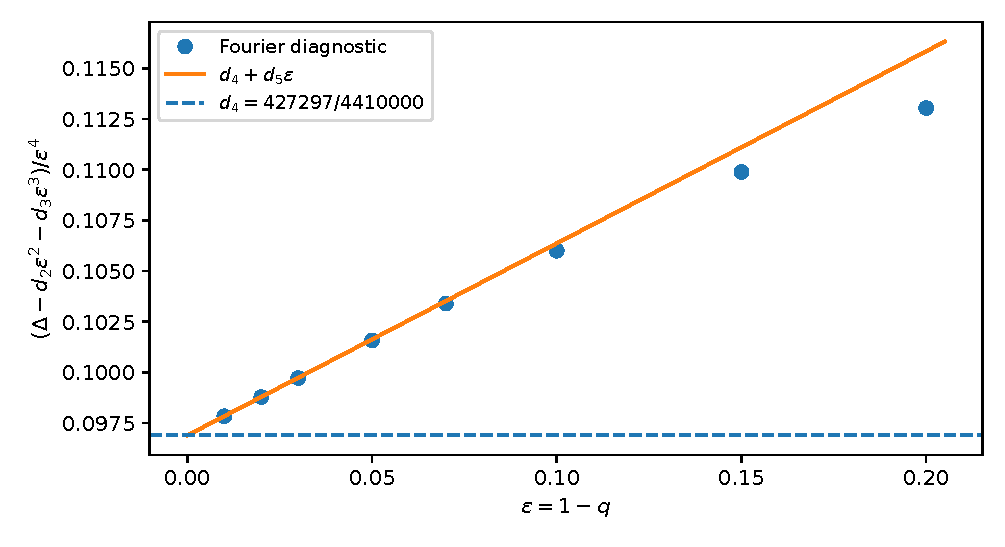
\includegraphics[width=.94\textwidth]{figures/quartic_check.pdf}
\caption{The quartic-scaled residual approaches the exact coefficient $d_4$.
Its first correction is $d_5\eps$. The analytic theorem, not this graph,
justifies the limit.}
\label{fig:quartic}
\end{figure}

\begin{figure}[htbp]
\centering
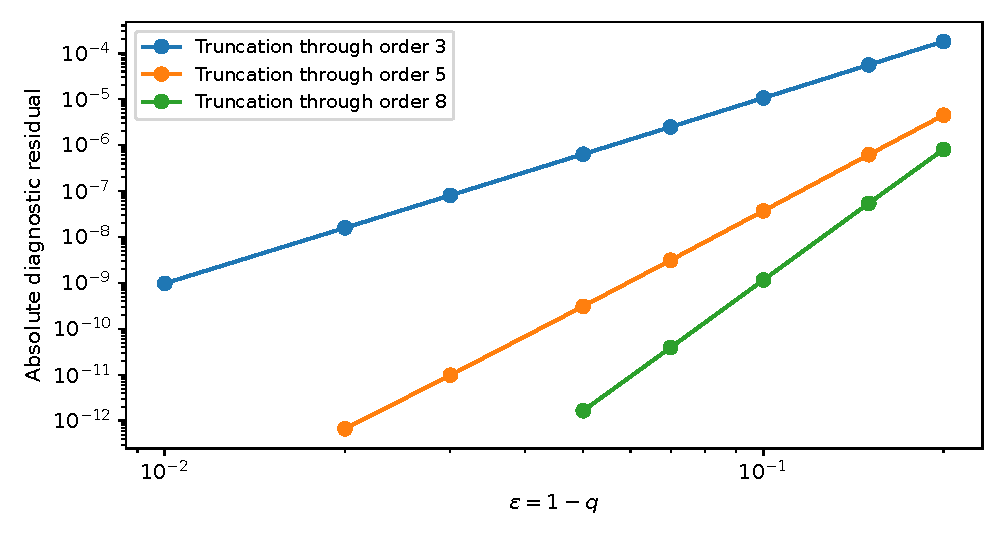
\includegraphics[width=.94\textwidth]{figures/truncation_errors.pdf}
\caption{Absolute residuals for three truncation orders. Values below
$10^{-13}$ are omitted to avoid presenting floating-point noise as an
asymptotic-rate measurement.}
\label{fig:errors}
\end{figure}

\subsection{Why the old numerical table is not an error certificate}

The targeted repository manuscript gives fixed-grid CDF-transfer estimates
$8.3866853\cdot10^{-5}$ at $q=0.95$ and
$2.8810502\cdot10^{-5}$ at $q=0.97$ \cite{repo}.
They differ visibly from the Fourier diagnostics above. We have not rerun that
original implementation and do not identify the discrepancy's cause here.
The practical conclusion is narrower: those earlier displayed values should
not be used as certified data for inferring fourth and higher coefficients.
The exact coefficient calculation and the proof of the remainder do not depend
on either numerical table.

\section{Proof audit and a formalization plan}
\label{sec:audit}

\subsection{Dependency structure}

The proof has two branches that meet only at the nonlinear transfer lemma.
The Fourier branch is
\[
 \text{comparable scales}
 \Longrightarrow\text{Fourier tails}
 \Longrightarrow\text{absolute density expansions}.
\]
The tail branch is
\[
 \text{uniform MGF bound}+\text{unimodality}+\text{bounded density}
 \Longrightarrow\text{Gaussian ratio envelope}.
\]
The transfer lemma combines them and gives Shannon and R\'enyi expansions.
The exact coefficient program is downstream of the cumulant formulas; it is
not used to establish any analytic estimate.

\begin{table}[htbp]
\centering
\small
\caption{Verification boundaries of the delivered package.}
\begin{tabular}{@{}p{.32\textwidth}p{.60\textwidth}@{}}
\toprule
Component & Status and evidence\\
\midrule
Repository conjecture & Exact source and label inspected at the pinned commit; no claim of a full repository audit.\\
Cumulant and Hermite algebra & Derived in the article; coefficients through degree eight replayed with exact rational arithmetic.\\
Fourier and tail estimates & Conventional proofs in Sections~\ref{sec:fourier}--\ref{sec:transfer}; no numerical assumptions.\\
Remainder uniformity & Explicit dependence restricted to fixed order, fixed $\rho_0<1$, and compact positive R\'enyi-order intervals.\\
Numerical table and figures & Reproducible floating-point diagnostics; not interval-certified.\\
Lean verification & Not performed; no new Lean theorem is claimed.\\
Publication priority & Targeted literature check only; general entropic Edgeworth theory is explicitly credited.\\
\bottomrule
\end{tabular}
\end{table}

\subsection{Natural formalization units}

A Lean development can separate finite algebra from analytic estimates rather
than encode the entire argument as one theorem. A sensible order is the
following.

First, formalize the moment-generating-function inequality for a uniform law,
including the elementary factorial comparison. Second, establish the
unimodality-to-density-envelope lemma abstractly for any density with a
variance-one Gaussian Chernoff bound. This lemma has no geometric-sum content
and is likely the most reusable analytic contribution of the proof.

Third, develop the comparable-scale block Fourier bound with explicit
constants and finite products, then pass to the infinite product. Fourth,
formalize the weighted-order polynomial algebra in
\eqref{eq:Aj}--\eqref{eq:recurrence}, including the distinction between the
linear Hermite map and multiplication. Fifth, prove a general nonlinear
transfer theorem from absolute density expansions and a polynomial Gaussian
envelope. Finally, instantiate the theorem for the Shannon and R\'enyi
integrands.

The rational identities are the easiest part to connect to executable
certificates. The difficult formal interfaces are Fourier inversion,
parameter-uniform asymptotic estimates, and domination of the information
integrals. The proof does not need a uniform positive lower bound for the
density, so a formalization should not introduce that false requirement.

\section{Further research questions}
\label{sec:questions}

The following questions distinguish genuine continuations from claims already
proved in this article.

\begin{problem}[Monotonic Gaussianization]
Is $q\mapsto D(Z_q\|\phi)$ strictly decreasing on the whole interval $(0,1)$?
The source manuscript states this separately from its Edgeworth conjecture
\cite{repo}. The expansion proved here does not settle it. In particular,
one must not differentiate an asymptotic expansion without proving a
derivative-stable remainder. A useful first target is such a derivative
estimate, which would imply strict monotonicity sufficiently near one.
\end{problem}

\begin{problem}[Infinite-order and growing-order divergence]
Determine $D_\infty(p_q\|\phi)=\log\sup_x p_q(x)/\phi(x)$, including the
location of maximizing points. The leading central polynomial is
$-H_4(x)/20$, whose maximum occurs at $x=\pm\sqrt3$, but the present
envelope alone does not exclude a remote competing maximum. More generally,
identify the transition when $\alpha=\alpha(\eps)\to\infty$.
\end{problem}

\begin{problem}[The nearly equal-weight finite-prefix regime]
Extend the two-parameter theorem to $\rho\uparrow1$ while $m\to\infty$.
A natural effective small parameter is
$(1-q^2)/(1-q^{2m})$. It is comparable to $1/m$ when $m(1-q)\to0$.
The desired theorem should interpolate between the iid uniform-sum expansion
and the infinite geometric expansion without coefficients blowing up in the
chosen coordinates.
\end{problem}

\begin{problem}[Effective constants and certified information computation]
Make $C_N$ and $\eps_N$ in \eqref{eq:main-estimate} explicit at useful
orders. Combine rational Taylor bounds, interval sinc products, and a
certified entropy quadrature. This would turn the asymptotic truncation rule
into an actual error-controlled numerical algorithm, rather than an
order-of-magnitude prescription.
\end{problem}

\begin{problem}[Coefficient growth and convergence]
Determine the large-$n$ growth of $d_n$ and $d_n(\alpha,0)$. Does the
Shannon series converge, diverge in a controlled Gevrey class, or require a
more general summation theory? The first eight coefficients cannot decide
this. Their sign changes also rule out relying on a naive positive-term
argument for monotonicity.
\end{problem}

\begin{problem}[Beyond-all-orders Shannon corrections]
Identify the exponentially small corrections to an optimally truncated
Shannon expansion. The order-zero support scale
$\sqrt\eps e^{-3/\eps}$ in \cref{cor:zero-order} is a concrete reference
scale, not a proved Shannon correction. Complex singularities of the sinc
product and saddle-point contributions may introduce different scales.
\end{problem}

\begin{problem}[Other digit distributions and nongeometric weights]
Find sharp assumptions on a symmetric digit law and a triangular array of
weights under which the same proof works. One needs an all-orders local
cumulant expansion, enough comparable coefficients for Fourier smoothing,
and a Gaussian-compatible information-tail bound. Boundedness alone does not
supply every one of these properties. A theorem for broad unimodal,
strictly subgaussian digit laws would isolate the real universality class.
\end{problem}

\begin{problem}[Fisher information and score expansions]
Prove an all-orders expansion for $J(p_q)-1$, where
$J(p)=\int(p')^2/p$. The derivative form of
\cref{thm:density-expansion} is only the central ingredient. The division by
$p$ makes the endpoint problem different from the forward R\'enyi case;
\eqref{eq:envelope} is an upper bound and is not sufficient by itself.
\end{problem}

\begin{problem}[A reusable formal nonlinear-asymptotic library]
Formalize \cref{lem:transfer} with an abstract compact parameter space and
explicit Gaussian polynomial integrability. Such a result would support
entropy, Hellinger, and other smooth divergence expansions well beyond this
single repository conjecture.
\end{problem}

\section{Conclusion}

The explicit entropic Edgeworth conjecture in the inspected \repo\ manuscript
is proved by \cref{thm:main}. The essential analytic addition is a uniform
method for carrying local Fourier expansions through a nonlinear information
integral despite compact support and moving endpoints. Its two components are
simple enough to audit separately: many comparable geometric scales suppress
high Fourier frequencies, while exact-variance subgaussianity and unimodality
bound the density ratio by a polynomial.

The same mechanism gives all finite positive R\'enyi orders and a uniform
finite-prefix expansion. Exact rational coefficients through degree eight,
an asymptotic prefix-length rule, and a sharp order-zero support scale make
the result concrete. Global entropy monotonicity, infinite-order divergence,
effective constants, and the double-scaling finite-prefix regime remain
separate, well-posed questions rather than consequences silently assumed here.

\appendix
\section{Exact Hermite product verification}
\label{app:hermite}

The product formula
\begin{equation}
 H_a(x)H_b(x)=\sum_{j=0}^{\min(a,b)}
  j!\binom aj\binom bj H_{a+b-2j}(x)
 \label{eq:hermite-product}
\end{equation}
follows by multiplying two generating functions in \eqref{eq:hermite} and
comparing coefficients. Orthogonality then gives
$\E H_a(G)H_b(G)=a!\,\mathbf1_{a=b}$.
For $a=b=4$,
\begin{equation}
 H_4^2=H_8+16H_6+72H_4+96H_2+24.
 \label{eq:H4-square}
\end{equation}
Thus $\E H_4^3=72\cdot4!=1728$,
$\E(H_4^2H_6)=16\cdot6!=11520$, and
$\E(H_4^2H_8)=8!=40320$. Squaring \eqref{eq:H4-square} and using
orthogonality gives
\[
 \E H_4^4=8!+16^2 6!+72^2 4!+96^2 2!+24^2=368064.
\]
The coefficient of $\lambda_4^4$ in \eqref{eq:invariant-fourth} is therefore
\[
 \frac1{24^4}\left(\frac{368064}{12}-\frac{40320}{8}\right)
 =\frac{89}{1152}.
\]
This independently exposes the small finite calculation behind the quartic
coefficient, without treating a computer algebra printout as its proof.

\section{Reproduction instructions}
\label{app:reproduce}

The archive is self-contained for compilation: the figure PDFs are already
included. From its root directory, run
\begin{lstlisting}
latexmk -pdf -interaction=nonstopmode -halt-on-error article.tex
\end{lstlisting}
To reproduce the exact arithmetic and floating-point diagnostics, use Python
with SymPy, NumPy, SciPy, and Matplotlib:
\begin{lstlisting}
python code/coefficients.py --order 8 --output data
python code/test_exact.py
python code/numerics.py --output data
python code/plots.py
\end{lstlisting}
The scripts were run with Python 3.13.5, SymPy 1.14.0, NumPy 2.3.5, and
SciPy 1.17.0; see the package's verification record for the exact environment.
The exact coefficient script needs only SymPy. The numerical and plotting
scripts are optional for reading or compiling the article.

For orientation, the algebraic core can be summarized as follows:
\begin{lstlisting}
for j = 1,...,N-1:
    A[j] = coefficient of epsilon^j in the cumulant log series
E[0] = 1
for n = 1,...,N-1:
    E[n] = sum(j*A[j]*E[n-j], j=1,...,n) / n
    P[n] = replace each z^k linearly by the Hermite polynomial H_k(x)
for n = 2,...,N:
    d[n] = coefficient of epsilon^n in
           GaussianExpectation(sum((-1)^k*U^k/(k*(k-1)), k=2,...,N))
    where U = sum(epsilon^j*P[j], j=1,...,N-1)
\end{lstlisting}
Every operation at a fixed order is finite. The growth of the amount of algebra
with $N$ does not enter the proof of the asymptotic remainder for a fixed $N$.

\begin{thebibliography}{9}
\bibitem{repo}
Vladimir Reshetnikov, \emph{ProveIt}, repository manuscript
\emph{Exact Information Geometry and New Frontiers for the Fabius--Rvachev
System}, especially the near-Gaussian section, conjecture
\texttt{conj:entropic-edgeworth}, and the numerical entropy table.
Inspected at commit \commit, 28 September 2026.\par
\url{https://github.com/VladimirReshetnikov/ProveIt/blob/6c9175a54bcaad3bfc2d416257d2b7d3dff2c1e0/Analysis/FabiusFunction/docs/semi-formalized-research-frontiers/drafts/inverse-and-sampling/fabius_information_frontier/fabius_information_frontier.tex}

\bibitem{arias}
Juan Arias de Reyna, \emph{Arithmetic of the Fabius function},
arXiv:1702.06487, version 3, 2017.\par
\url{https://arxiv.org/abs/1702.06487}

\bibitem{bcg2013}
Sergey G. Bobkov, Gennadiy P. Chistyakov, and Friedrich G\"otze,
\emph{Rate of convergence and Edgeworth-type expansion in the entropic central
limit theorem}, Annals of Probability \textbf{41} (2013), no.~4, 2479--2512.
DOI: 10.1214/12-AOP780; arXiv:1104.3994.\par
\url{https://arxiv.org/abs/1104.3994}

\bibitem{bcg2016}
S. G. Bobkov, G. P. Chistyakov, and F. G\"otze,
\emph{R\'enyi divergence and the central limit theorem},
arXiv:1608.01805, 2016.\par
\url{https://arxiv.org/abs/1608.01805}

\bibitem{bcg2025}
S. G. Bobkov, G. P. Chistyakov, and F. G\"otze,
\emph{R\'enyi Divergences in Central Limit Theorems: Old and New},
arXiv:2503.03926, 2025.\par
\url{https://arxiv.org/abs/2503.03926}
\end{thebibliography}
\end{document}
